\documentclass[11pt]{article}
\usepackage[margin=1in]{geometry}
\usepackage{graphicx,amsmath,booktabs,xcolor}
\usepackage[T1]{fontenc}
\usepackage{mathptmx}
\usepackage[authoryear,round]{natbib}
\usepackage[colorlinks=true,citecolor=blue!50!black,linkcolor=blue!50!black,urlcolor=blue!50!black]{hyperref}
\bibliographystyle{plainnat}
\title{An I-band Period--Luminosity Distance to the Globular Cluster Kestrel-7 from 42 RR Lyrae Stars}
\author{Bianca Azartash\\ \small University of Oklahoma Libraries, Norman, OK, USA}
\date{Draft of 30 October 2026}

\begin{document}
\maketitle
\begin{center}\fbox{\parbox{0.92\textwidth}{\small\color{red!60!black}\textbf{DRAFT PREPRINT --- MOCK RESEARCH PROJECT. All data are synthetic and Kestrel-7 is a fictional cluster. Cited works marked as fictional in references.bib do not exist.}}}\end{center}
\begin{abstract}
We present V- and I-band time-series photometry of 42 RR Lyrae stars in the recently discovered globular cluster Kestrel-7 \citep{haddad2021}. Using Lomb--Scargle periodograms and fourth-order Fourier fits, we identify 28 fundamental-mode (RRab) and 14 first-overtone (RRc) pulsators. The mean RRab period, $\langle P_{ab}\rangle = 0.593$ d, places Kestrel-7 in the Oosterhoff gap. A free fit to the I-band period--luminosity relation gives a slope of $-1.23 \pm 0.09$, consistent with recent calibrations. Adopting the parallax-based calibration of \citet{okafor2023} and a reddening of $E(B-V) = 0.08$ \citep{chen2024}, we derive a true distance modulus of $\mu_0 = 15.11 \pm 0.01$ (stat) $\pm 0.07$ (sys) mag, corresponding to $10.5 \pm 0.3$ kpc.
\end{abstract}

\section{Introduction}
RR Lyrae stars are low-mass, core-helium-burning pulsators that trace old stellar populations. Although their V-band absolute magnitudes depend only weakly on period, a well-defined period--luminosity (PL) relation appears at redder wavelengths, where the relation is also less sensitive to metallicity and interstellar extinction \citep{okafor2023}. This makes I-band RR Lyrae photometry an efficient distance indicator for globular clusters.

Kestrel-7 was identified as a compact overdensity behind the southern Galactic bulge, with a horizontal-branch distance of $11 \pm 2$ kpc \citep{haddad2021}. Variability among horizontal-branch stars in the discovery data motivated the dedicated time-series campaign presented here. Our goals are to (i) build a clean RR Lyrae census, (ii) determine the cluster's Oosterhoff type, and (iii) measure a precise PL distance.


\section{Observations and Data Reduction}
We obtained 62 epochs in each of V and I over a 118-day baseline. Point-spread-function photometry was performed on all frames and calibrated to a standard system. Each light curve was inspected and epochs flagged by the reduction pipeline (cosmic rays, bad columns; 25 of 5208 measurements) were removed. The resulting photometry is provided in \texttt{data/raw/kestrel7\_photometry.csv}. Typical uncertainties are 0.01--0.02 mag.


\section{Analysis}
Periods were determined from the V-band data with a Lomb--Scargle periodogram \citep{lomb1976,scargle1982} over 0.2--1.0 d. We inspected folded light curves at the strongest peaks to rule out daily aliases, a common failure mode for nightly sampling \citep{petrov2019}. Phased light curves in each band were fit with a fourth-order Fourier series, and mean magnitudes were computed by intensity-averaging the fitted model \citep{petrov2019}. Example light curves are shown in Figure~\ref{fig:3}.

Stars with $P < 0.43$ d and sinusoidal light curves were classified as RRc. Their periods were fundamentalized with $\log P_F = \log P + 0.127$. The resulting period--amplitude (Bailey) diagram (Figure~\ref{fig:2}) shows two clean sequences with no ambiguous objects.

We fit $\langle I \rangle = a \log P_F + b$ by least squares, and separately derived $\mu_0$ by fixing the slope and zero point to the calibration $M_I = -1.13 \log P_F + 0.47$ \citep{okafor2023}, correcting for $A_I = 0.15$ mag. Statistical uncertainties were estimated with 2000 bootstrap resamples. The analysis code is \texttt{src/rrlyrae\_pl.py}, and a step-by-step record is in \texttt{notebooks/kestrel7\_analysis.ipynb}.

\begin{figure}[t]
\centering
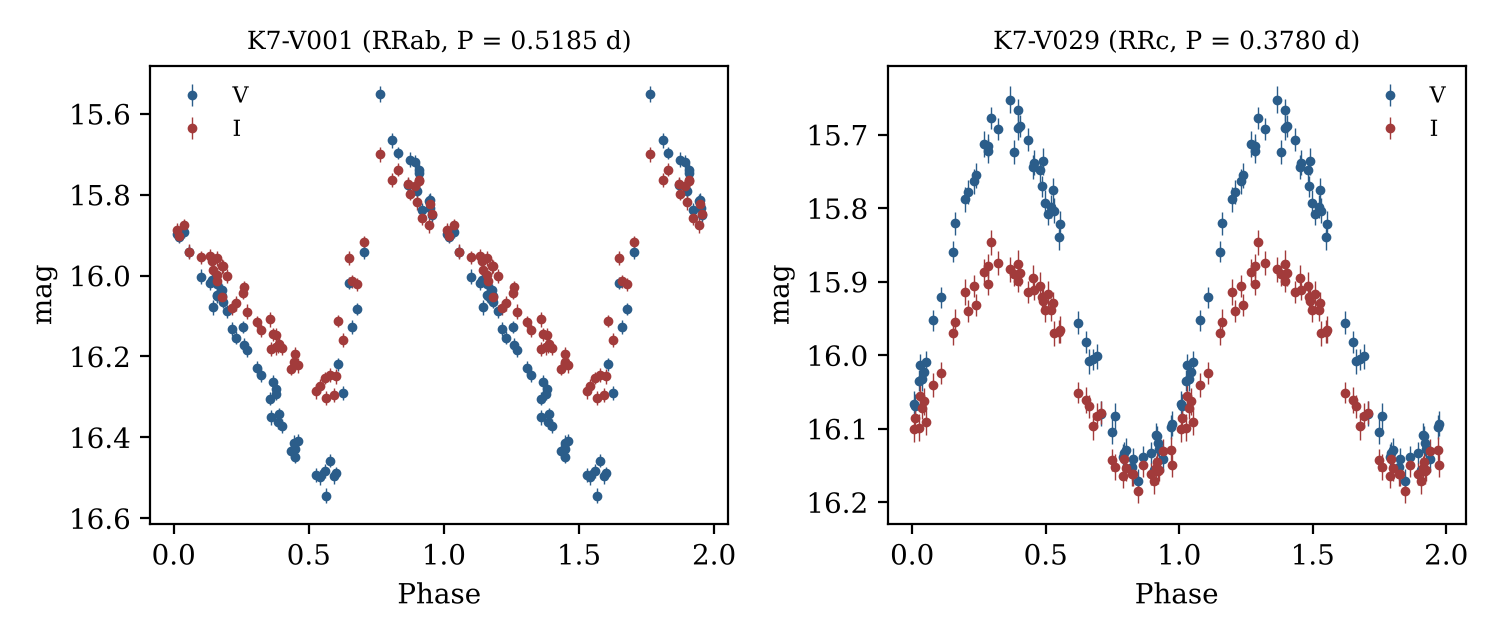
\includegraphics[width=0.95\textwidth]{figures/fig3_example_lightcurves.png}
\caption{Example phased V- and I-band light curves for one RRab and one RRc star, plotted over two cycles.}\label{fig:3}
\end{figure}
\begin{figure}[t]
\centering
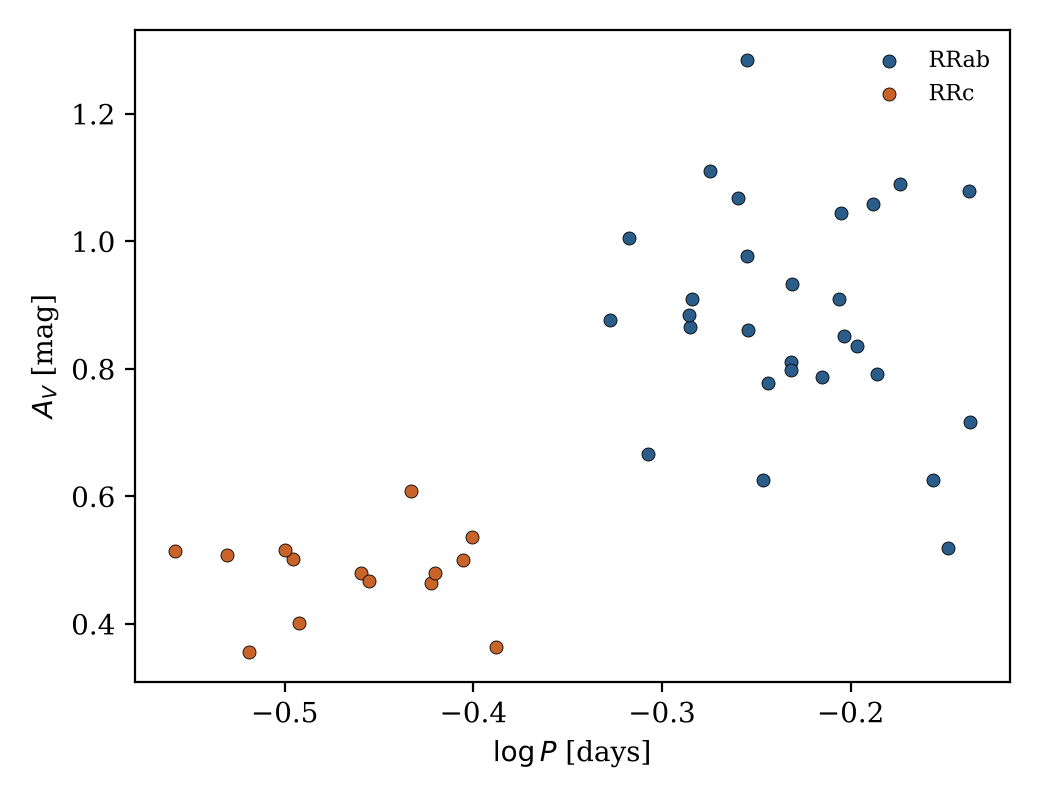
\includegraphics[width=0.62\textwidth]{figures/fig2_bailey_diagram.png}
\caption{Bailey (period--amplitude) diagram. RRab and RRc stars form two distinct sequences.}\label{fig:2}
\end{figure}

\section{Results}
Our final catalog contains 28 RRab and 14 RRc stars (Table~\ref{tab:1}). The mean RRab period is $\langle P_{ab}\rangle = 0.593$ d and the mean RRc period is $\langle P_c\rangle = 0.347$ d, with an RRc fraction of 0.33.

The free-slope PL fit (Figure~\ref{fig:1}) gives $a = -1.23 \pm 0.09$ and $b = 15.70 \pm 0.03$ with an rms scatter of 0.043 mag, consistent with the intrinsic scatter of the calibrating relation. With the slope fixed to the calibration, we find $\mu_0 = 15.11 \pm 0.01$ (stat) $\pm 0.07$ (sys) mag, or $d = 10.5 \pm 0.3$ kpc.

\begin{table}[t]
\centering
\caption{Summary of derived properties of Kestrel-7.}\label{tab:1}
\begin{tabular}{ll}
\toprule
Quantity & Value \\
\midrule
RRab / RRc & 28 / 14 \\
$\langle P_{ab}\rangle$ & 0.593 d \\
$\langle P_c\rangle$ & 0.347 d \\
PL slope (free) & $-1.23 \pm 0.09$ \\
PL rms scatter & 0.043 mag \\
$A_I$ & 0.15 mag \\
$\mu_0$ & $15.11 \pm 0.01$ (stat) $\pm 0.07$ (sys) \\
Distance & $10.5 \pm 0.3$ kpc \\
\bottomrule
\end{tabular}
\end{table}
\begin{figure}[t]
\centering
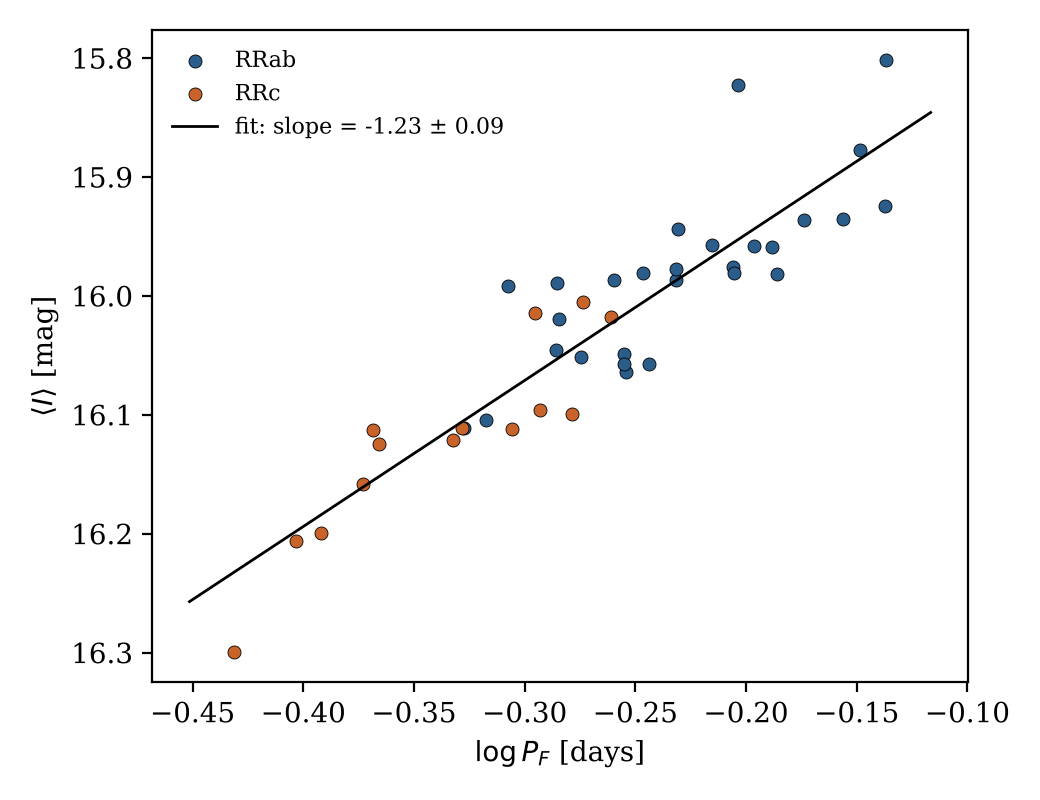
\includegraphics[width=0.62\textwidth]{figures/fig1_pl_relation_I.png}
\caption{I-band period--luminosity relation for Kestrel-7. RRc periods are fundamentalized. The line shows the free least-squares fit.}\label{fig:1}
\end{figure}

\section{Discussion}
Our distance agrees with, and is roughly six times more precise than, the horizontal-branch estimate of \citet{haddad2021}. The error budget is dominated by the systematic terms: the calibration zero point (0.05 mag) and the reddening (0.02 mag in $E(B-V)$, or about 0.04 mag in $A_I$).

With $\langle P_{ab}\rangle = 0.593$ d, Kestrel-7 falls in the 0.58--0.62 d range that is sparsely populated among Galactic halo clusters \citep{moreau2022}. Its RRc fraction (0.33) is also intermediate between typical Oosterhoff I and II values. Oosterhoff-intermediate clusters are often associated with accreted systems, which makes Kestrel-7 a promising target for spectroscopic metallicity and kinematic follow-up.


\section{Conclusions}
We have identified 42 RR Lyrae stars in Kestrel-7 and used their I-band PL relation to measure a distance of $10.5 \pm 0.3$ kpc. The cluster is Oosterhoff-intermediate. Planned future work includes spectroscopic metallicities, which will allow us to apply a metallicity-dependent PL calibration.


\section*{Acknowledgments}
This draft is part of a mock research project created for teaching and documentation exercises. No real telescope time was used.

\bibliography{references}

\end{document}
